% This is "sig-alternate.tex" V1.9 April 2009
% This file should be compiled with V2.4 of "sig-alternate.cls" April 2009
%
% This example file demonstrates the use of the 'sig-alternate.cls'
% V2.4 LaTeX2e document class file. It is for those submitting
% articles to ACM Conference Proceedings WHO DO NOT WISH TO
% STRICTLY ADHERE TO THE SIGS (PUBS-BOARD-ENDORSED) STYLE.
% The 'sig-alternate.cls' file will produce a similar-looking,
% albeit, 'tighter' paper resulting in, invariably, fewer pages.
%
% ----------------------------------------------------------------------------------------------------------------
% This .tex file (and associated .cls V2.4) produces:
%       1) The Permission Statement
%       2) The Conference (location) Info information
%       3) The Copyright Line with ACM data
%       4) NO page numbers
%
% as against the acm_proc_article-sp.cls file which
% DOES NOT produce 1) thru' 3) above.
%
% Using 'sig-alternate.cls' you have control, however, from within
% the source .tex file, over both the CopyrightYear
% (defaulted to 200X) and the ACM Copyright Data
% (defaulted to X-XXXXX-XX-X/XX/XX).
% e.g.
% \CopyrightYear{2007} will cause 2007 to appear in the copyright line.
% \crdata{0-12345-67-8/90/12} will cause 0-12345-67-8/90/12 to appear in the copyright line.
%
% ---------------------------------------------------------------------------------------------------------------
% This .tex source is an example which *does* use
% the .bib file (from which the .bbl file % is produced).
% REMEMBER HOWEVER: After having produced the .bbl file,
% and prior to final submission, you *NEED* to 'insert'
% your .bbl file into your source .tex file so as to provide
% ONE 'self-contained' source file.
%
% ================= IF YOU HAVE QUESTIONS =======================
% Questions regarding the SIGS styles, SIGS policies and
% procedures, Conferences etc. should be sent to
% Adrienne Griscti (griscti@acm.org)
%
% Technical questions _only_ to
% Gerald Murray (murray@hq.acm.org)
% ===============================================================
%
% For tracking purposes - this is V1.9 - April 2009

\documentclass{sig-alternate}

\usepackage{url}
\usepackage{algorithm,algorithmic}
\DeclareMathOperator*{\dist}{dist}
\DeclareMathOperator*{\size}{size}


\begin{document}
%
% --- Author Metadata here ---
\conferenceinfo{ACM Multimedia}{2010 Firenze, Italy}
\CopyrightYear{2010} % Allows default copyright year (200X) to be over-ridden - IF NEED BE.
\crdata{0-12345-67-8/90/01}  % Allows default copyright data (0-89791-88-6/97/05) to be over-ridden - IF NEED BE.
% --- End of Author Metadata ---

\title{Towards the Infinite Listening Machine}
%\subtitle{[Extended Abstract]
%\titlenote{A full version of this paper is available as
%\textit{Author's Guide to Preparing ACM SIG Proceedings Using
%\LaTeX$2_\epsilon$\ and BibTeX} at
%\texttt{www.acm.org/eaddress.htm}}}

%
% You need the command \numberofauthors to handle the 'placement
% and alignment' of the authors beneath the title.
%
% For aesthetic reasons, we recommend 'three authors at a time'
% i.e. three 'name/affiliation blocks' be placed beneath the title.
%
% NOTE: You are NOT restricted in how many 'rows' of
% "name/affiliations" may appear. We just ask that you restrict
% the number of 'columns' to three.
%
% Because of the available 'opening page real-estate'
% we ask you to refrain from putting more than six authors
% (two rows with three columns) beneath the article title.
% More than six makes the first-page appear very cluttered indeed.
%
% Use the \alignauthor commands to handle the names
% and affiliations for an 'aesthetic maximum' of six authors.
% Add names, affiliations, addresses for
% the seventh etc. author(s) as the argument for the
% \additionalauthors command.
% These 'additional authors' will be output/set for you
% without further effort on your part as the last section in
% the body of your article BEFORE References or any Appendices.

\numberofauthors{3} %  in this sample file, there are a *total*
% of EIGHT authors. SIX appear on the 'first-page' (for formatting
% reasons) and the remaining two appear in the \additionalauthors section.
%
\author{
% You can go ahead and credit any number of authors here,
% e.g. one 'row of three' or two rows (consisting of one row of three
% and a second row of one, two or three).
%
% The command \alignauthor (no curly braces needed) should
% precede each author name, affiliation/snail-mail address and
% e-mail address. Additionally, tag each line of
% affiliation/address with \affaddr, and tag the
% e-mail address with \email.
%
% 1st. author
\alignauthor
Ben Trovato\titlenote{Dr.~Trovato insisted his name be first.}\\
       \affaddr{Institute for Clarity in Documentation}\\
       \affaddr{1932 Wallamaloo Lane}\\
       \affaddr{Wallamaloo, New Zealand}\\
       \email{trovato@corporation.com}
% 2nd. author
\alignauthor
G.K.M. Tobin\\
       \affaddr{Institute for Clarity in Documentation}\\
       \affaddr{P.O. Box 1212}\\
       \affaddr{Dublin, Ohio 43017-6221}\\
       \email{webmaster@marysville-ohio.com}
% 3rd. author
\alignauthor Lars Th{\o}rv{\"a}ld\\
       \affaddr{The Th{\o}rv{\"a}ld Group}\\
       \affaddr{1 Th{\o}rv{\"a}ld Circle}\\
       \affaddr{Hekla, Iceland}\\
       \email{larst@affiliation.org}
% REAL AUTHORS:
%\alignauthor
%Thierry Bertin-Mahieux\\
%       \affaddr{Columbia University}\\
%       \affaddr{New York, USA}\\
%       \email{tb2332@columbia.edu}
% 2nd. author
%\alignauthor
%Ron Weiss\\
%       \affaddr{New York University}\\
%       \affaddr{New York, USA}\\
%       \email{ronw@nyu.edu}
% 3rd. author
%\alignauthor Dan Ellis\\
%       \affaddr{Columbia University}\\
%       \affaddr{New York, USA}\\
%       \email{dpwe@ee.columbia.edu}
%\and  % use '\and' if you need 'another row' of author names
% 4th. author
%\alignauthor Lawrence P. Leipuner\\
%       \affaddr{Brookhaven Laboratories}\\
%       \affaddr{Brookhaven National Lab}\\
%       \affaddr{P.O. Box 5000}\\
%       \email{lleipuner@researchlabs.org}
}
% There's nothing stopping you putting the seventh, eighth, etc.
% author on the opening page (as the 'third row') but we ask,
% for aesthetic reasons that you place these 'additional authors'
% in the \additional authors block, viz.
%\additionalauthors{Additional authors: John Smith (The Th{\o}rv{\"a}ld Group,
%email: {\texttt{jsmith@affiliation.org}}) and Julius P.~Kumquat
%(The Kumquat Consortium, email: {\texttt{jpkumquat@consortium.net}}).}
\date{7 May 2010}
% Just remember to make sure that the TOTAL number of authors
% is the number that will appear on the first page PLUS the
% number that will appear in the \additionalauthors section.

\maketitle
\begin{abstract}
Any subset of data is a limitation unrelated to reality. Multimedia data
is abundant, infinite in regard to any human being. Human learning is not
bounded by data sizes, even if some samples (artists, shows, etc) appear
more often. In this work we build a framework for online learning over
``infinite'' audio data. We show how to handle a stream
of non stop music, analyze it, and learn from it. 
We focus on the clustering and
the encoding of music harmonic patterns as it can gives us a representation
of the whole music space. Nevertheless, the end goal is to build a
system that, similar to humans, will ``hear'' new sounds and learn from
it in an online fashion without any upper bound on the amount of data.

We use an online vector quantization algorithm to learn a codebook.
Samples are taken live from an online music feature provider, but we
show how to reproduce the features from a live stream of audio.

``If your data fits in memory, you need more data.''
\end{abstract}


% A category with the (minimum) three required fields
\category{H.4}{Information Systems Applications}{Miscellaneous}
%A category including the fourth, optional field follows...
\category{D.2.8}{Software Engineering}{Metrics}[complexity measures, performance measures]

\terms{Theory}

\keywords{Online Machine Learning, Music Information Retrieval}

\section{Introduction}
JNMR with filterboost: \cite{Bertin-Mahieux2008}. 
Chroma features \cite{Casey2006,Casey2008,Ellis2007}.
Learn from harmonic data: \cite{Anglade2009}.
EchoNest \cite{EchoNest}.
Beat tracking \cite{Ellis2007b}.
Information theory: \cite{Cover1991}.

Scaling is awesome. In multimedia, e.g. audio and video, we have an
inifinite source of data available through the web. We set ourselves
to harness this endless data through a simple and memory efficient
algorithm.

We want to learn about the data, and eventually even learn how it
changes in time. We add a filtering componet to our framework
to make it focus on new and original data.


\section{Framework}
trainer - model - oracle

Our model can be split into $3$ distinct parts: the model, the oracle,
and the trainer. The oracle is solely responsible to gathering data.
In our ``infinite'' implementation, it queries an online service or
analyze live streams. For testing reason, the oracle can gather data
saved on disk.

The model is an online learning algorithm that receives a few samples
an a time (usually coming from one song) and updates itself accordingly.

The trainer glue things together. It can select the batch size passed
to the model, filter the samples, and keep track of the performance of
the model.

Scaling is the main concern of this work. Thus we restrain ourselves
from forming large batches of training samples. Our algorithm should be
$O(n)$ with $n$ number of samples seen if we do not want to be contrived
by any upper limit. Time is always an issue but memory should not be.


\section{Audio Sources}
Echo Nest is a big one. With $5$ threads, we gather approximately one song
every $3$ seconds.

Downloaded data.

Audio stream. Then upload to Echo Nest or reproduce the results. Works
but slow.

\section{Learning Codebook}

See Figure \ref{fig:encodesong}.

\begin{figure}[thb]
\begin{center}
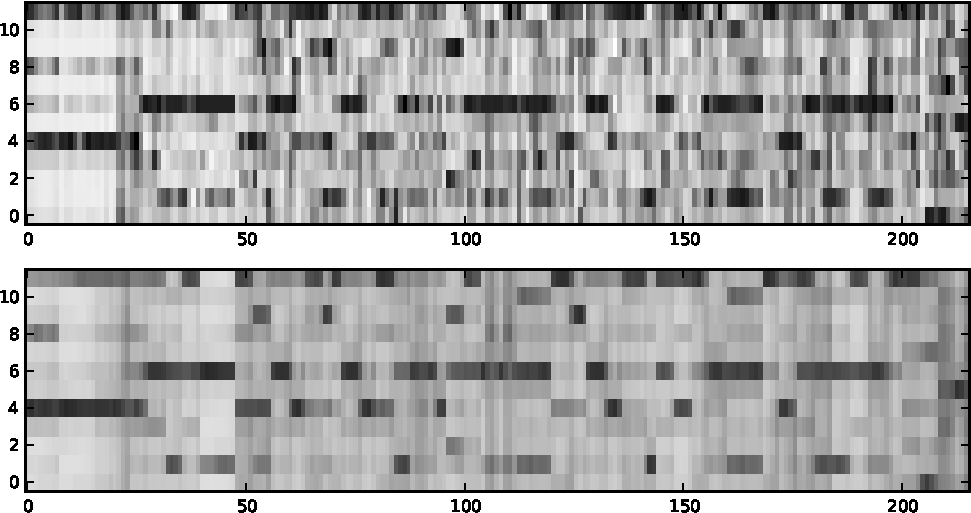
\includegraphics[width=.9\columnwidth]{song_encoded}
\end{center}
\caption{\small{Good Day Sunshine by \textit{The Beatles}.
Original song and encoding with a $200$ entry codebook of 
$2$ bar patterns.
}}
\label{fig:encodesong}
\end{figure}

\subsection{Data}
Echo Nest API \cite{EchoNest} is great, but it is easy to reproduce
the analysis using a beat tracker and chromas. The bar analysis is
more trickier, however it can be learned\footnote{citation omitted to preserve 
anonymity}. Not that most of the bars are made of $4$ beats and less
than $10$ are not $3$ or $4$ beat-long bars.

EchoNest is reported to have millions of tracks analyzed. We datamined
the artist to get a set of $200$K of them. Out of our large artist set,
we confirmed for $70$K that they have tracks analyzed (with an average
of ... track per artist). Thus, our oracle chooses randomly from a set of
$2$M? tracks, but it is not a limitation. Note that new tracks are added
daily to the Echo Nest service.

For EN, the average of artists having at least one song is ... For those
artists, the average number of songs (upper bounded to $100$) is ...
An average song has ... bars.


The feature analysis used throughout this work is based on Echo Nest
analyze API \cite{EchoNest}.  
%
For any song uploaded to their platform this analysis returns a chroma
vector (length $12$) for every music event (called ``segment''), and a
segmentation of the song into beats and bars. Beats may span or 
subdivide segments; bars span multiple beats.
%
Averaging the per-segment chroma over beat times results in a
beat-synchronous chroma feature representation similar to that used in
\cite{Ellis2007a}.  Echo Nest chroma vectors are normalized to have the 
largest value in each column equal to 1.

% \begin{figure}[htb]
% \begin{center}
% \includegraphics[width=.9\columnwidth]{bar_size_freq}
% \end{center}
% \caption{\small{
% Frequency of the different bar size in the training data.
% }}
% \label{fig:barsize}
% \end{figure}

Note that none of this information (segments, beats, bars)
can be assumed perfectly accurate.
%(\eg in \cite{Barrington2009a} authors obtain a better
%song segmentation than the Echo Nest). 
In practice, we have found them reasonable, 
and given the size of the data set, any rare imperfections or noise
can be diluted to irrelevance by the good examples.  
We also believe that patch sizes based on a number of beats or bars are more
meaningful than an arbitrary time length.


\subsubsection{Beat-Chroma Patches} \label{ssec:beatpatch}

We use the bar segmentation obtained from the Echo Nest analysis to
break a song into a collection of beat-chroma ``patches'', typically
one or two bars in length.
Because the bar length is not guaranteed to be 4 beats, 
depending on the meter of a particular
song, we resample each patch to a fixed length of 4 beats
per bar (except where noted).  However, the majority (82\%) of our training data
consisted of bars that were 4 beats long, so this resampling 
usually had no effect.  Most of the remaining bars (10\%) were 3 beats in
length.
The resulting patches consist of $12 \times 4$ or $12 \times 8$ matrices.

Finally, we normalize the patches with respect to transposition by rotating
the pattern matrix so that the first row contains the most
energy. This can be seen in the example codeword of Figure ...
Each patch within a song is normalized independently, so
reconstruction of the original song requires knowledge of the
rotation index (key) for each patch.

The representation resulting from this process is invariant to both
the key and meter of the original song.  This enables the study of
broad harmonic patterns found throughout the data, without regard for
the specific musical context.
In the context of clustering this avoids problems such as obtaining separate
clusters for every major triad for both duple and triple meters.

\subsection{Vector Quantization}
We use an online version of the vector quantization algorithm
\cite{Gersho1991} to cluster the beat-chroma patches described in the
previous section.
For each sample from the data, the algorithm finds the closest cluster
in the codebook and updates the cluster centroid (codeword) to be
closer to the sample according to a learning rate $\ell$.
The clusters are updated as each data point is seen, as opposed to
once per iteration in the standard $k$-means algorithm.
The details are explained in Algorithm \ref{algo:vq}.
%
As in standard $k$-means clustering, the codebook is initialized by
choosing $K$ random points from our dataset.

\begin{algorithm}
%\caption{Pseudocode of Vector Quantization}
\begin{algorithmic}
\STATE$\ell$ learning rate
\STATE$\{P_n\}$ set of patches
\STATE$\{C_k\}$ codebook of $K$ codes
%\STATE $m \leftarrow b$
\REQUIRE $0 < \ell \leq 1$
\FOR{$nIters$}
\FOR{$p \in \{P_n\}$}
\STATE$c \leftarrow \min_{c \in C_k} \dist(p,c)$
\STATE$c \leftarrow c + (p - c) * \ell$
\ENDFOR
\ENDFOR
\RETURN $\{C_k\}$
\caption{\small{Pseudocode for the online vector quantization
    algorithm.}\label{algo:vq}}
\end{algorithmic}
\end{algorithm}


\subsection{Large Data Learning}
One problem is the convergence of the learning algorithm. It is normal
that an algorithm learns more from the first first example than from the
millionth one. However, our algorithm should remain capable of learning
from an original new sample, e.g. an outlier. We introduce filtering
for that purpose.


\section{Applications}
We present applications of our particular encoding, i.e. representing
a song as a set of chroma patches. Note that the framework in this
paper could be use for other types of features or patches. For instance
patches preserving timbral information, such as MFCC patches.

In \cite{Casey2006} authors show that such encoding can be used for
cover recognition. In other work\footnote{in press; reference hidden
to preserve submissions's anonymity}, authors show that harmonic codewords
retain information about bar alignment and artist recognition.

\subsection{Bitrate}

We focus on showing that our algorithm learns the encoding correctly.
We study the distortion on new songs for different encoding rates.
Since music is not a random signal and contains meaningful repetitions,
longer codewords for a given bitrate should perform better. The downsize
is that longer codewords mean more of them to keep the bitrate constant,
and more codewords implies a longer learning. As we mentioned earlier,
training on an ever increasing number of samples is challenging.

See Figure \ref{fig:bitrates}.

\begin{figure}[thb]
\begin{center}
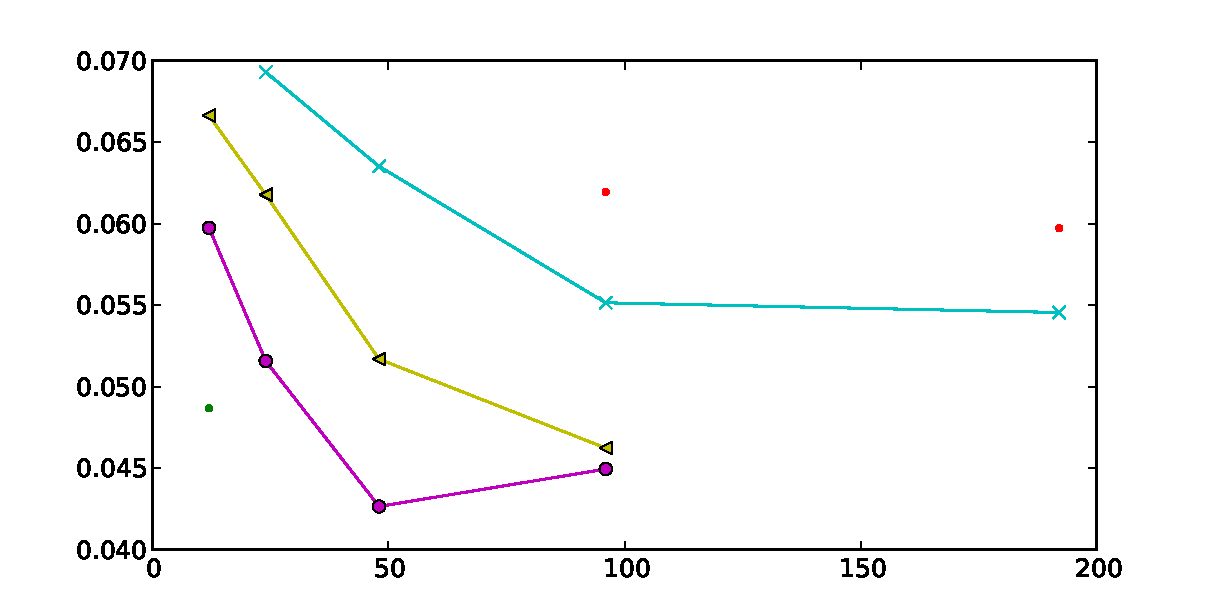
\includegraphics[width=.9\columnwidth]{bitrates}
\end{center}
\caption{\small{Different bitrates blah blah blah.
}}
\label{fig:bitrates}
\end{figure}

\subsection{Filtering}
We compare the learning of a codebook of size $100$, 2 bars represented
as 8 beats, key invariance over patches. The filtering learning
takes indeed more time as many samples are discarded.

See Figure \ref{fig:filt}.

\begin{figure}[thb]
\begin{center}
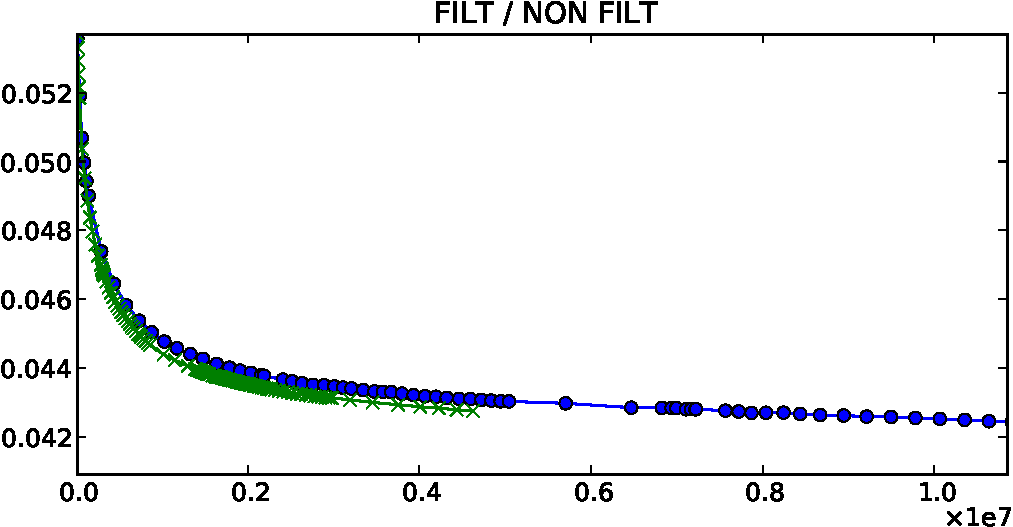
\includegraphics[width=.99\columnwidth]{filt_nonfilt}
\end{center}
\caption{\small{
Learning curve with and without filtering. $100$ codewords learn for
patterns spanning $2$ bars with $8$ beats. Learning dataset is the
whole Echo Nest collection.
}}
\label{fig:filt}
\end{figure}

\section{Conclusion and Future Work}
We have presented the framework and a first implementation of what
we call the ``Infinite Listening Machine''. The algorithms learns from
an infinite source of data in an online fashion. We have defined a
possible set of features and one algorithm that meats our requirements.
We showed through some application that it is a viable learning scheme.
Finally, we gave many directions for improvement and future works.

Future work includes online NMF, GMM, neural networks.

Train model restrained to given metadata, such as release year.
Model new trends, for instance the increasing use of distortion
since the $50$'s.

%ACKNOWLEDGMENTS are optional
%\section{Acknowledgments}
%Thierry has a grant. Ron too.

%
% The following two commands are all you need in the
% initial runs of your .tex file to
% produce the bibliography for the citations in your paper.
\bibliographystyle{abbrv}
\bibliography{tbm_bib}  % sigproc.bib is the name of the Bibliography in this case
% You must have a proper ".bib" file
%  and remember to run:
% latex bibtex latex latex
% to resolve all references
%
\end{document}
